\section{Problem statement}

The technical problem we are addressing in this assignment is the process of tracking features of a human eye in video data.\\
The human eye is perhaps a persons most important sensory organ, and as such identification of eye features has many applications. 
\begin{itemize}
	\item The movement of the eye, being indicative of the direction in which the person is looking, can be used in determining what a person pays attention to in a given situation.
	\item Some security systems rely on scanning the unique features of the eye to determine a persons identity.
	\item Humans look at the features and movement of each others eyes to determine the others emotional state and thought processes; it might be possible for machines to replicate this process.
\end{itemize}

In this assignment we will simply attempt to identify the position of certain eye features. We will perform no further analysis of these features, such as deriving meaning from their relative position and movement.\\

The features we are trying to locate are:
\begin{enumerate}
	\item[Pupil] The pupil is the large, round black spot in the center of the eye. This is one of the eye's most distinctive features.
	\item[Glints] The glints are small bright spots caused by reflection of light in the eye's surface. They are usually found close to the pupil, and those close to the pupil are the most pronounced. 
	\item[Iris] The iris, or limbus, is the colorful round section surrounding the pupil. It is usually partially covered by the eyelids. 
\end{enumerate}

\begin{figure}[h]
	\centering
	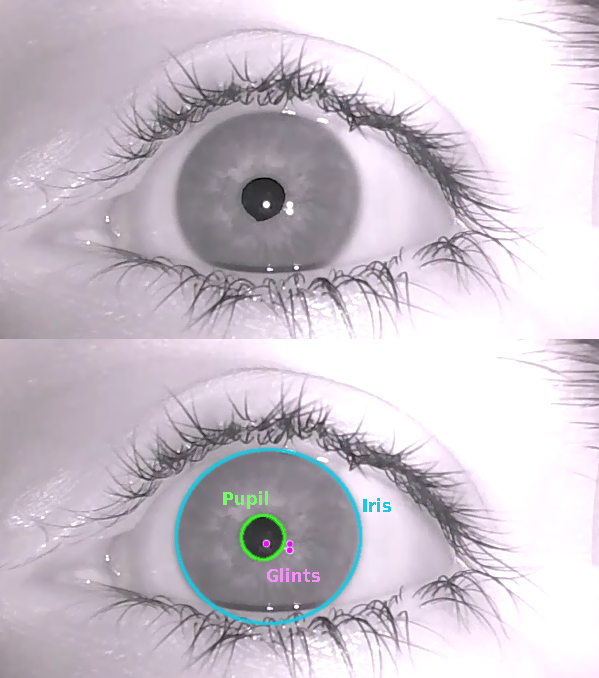
\includegraphics[scale=0.6]{eye_terms.png}
	\caption{The eye features we wish to identify}
\end{figure}

Other pronounced features of the eye are the eyelids, eyelashes and eye corners. These are more complex shapes, and are more difficult to locate precisely. They will not be the focus of this assignment.\\

\subsection{Test Data}
	A set of test data have been provided to aid the assignment. These include 12 video files named from "eye1.avi" to "eye12.avi", containing close-up video recordings of human eyes in a variety of conditions; brightness level, size of the eye and movement patterns vary. These are intended to offer proper challenges to our tracking solution, to ensure that it works in less-than-perfect recording conditions. A final recording named "EyeBizaro.avi" contains one particularly difficult recording, where the eye moves around wildly under extreme lighting conditions.\\
	
	The recordings are in black and white, meaning that we cannot extract color information from the videos. We cannot, for instance, filter out colorful sections in an attempt to locate the iris.\\
	
	In our solution we will treat these videos only as sequences of still frames, and carry out all analysis with the assumption that we are working with still images.\\
	
	When assessing the functionality of our solution we will not assume that a satisfying solution is one that can identify all relevant eye features in all recordings. We will consider the solution satisfactory if it identifies the correct features and only those in a majority of the frames of each video. Our solution will thus be focused not on demanding that we locate the correct number of each feature, but simply on reducing the number of false positive and negative detections as much as possible with the available techniques. 